\documentclass[a4paper,11pt]{report}

\usepackage[ngerman]{babel}

% LAYOUT & FORMATTING ----------------------------------
\usepackage{geometry}
\geometry{a4paper, top=25mm, left=35mm, right=20mm, bottom=25mm, headsep=10mm, footskip=12mm}
\usepackage[utf8]{inputenc}
\usepackage[T1]{fontenc}

\usepackage{amssymb}

\usepackage{listings}
% ------------------------------------------------------

% IMAGES AND PLOTS -------------------------------------
\usepackage{graphicx}
\usepackage{tikz}
\usetikzlibrary{patterns, snakes, shapes.misc, positioning}
% cache tikz images
%\usepackage{shellesc}
%\usetikzlibrary{external}
% name of the folder where images are cached (create folder by yourself)
%\tikzexternalize[prefix=tikz/]
% ------------------------------------------------------

% COMMANDS ---------------------------------------------
\newcommand{\fref}[1]{Abbildung~\ref{#1}}
\newcommand{\sref}[1]{Abschnitt~\ref{#1}}
\newcommand{\cref}[1]{Kapitel~\ref{#1}}

\newcommand{\titleofcard}[1]{\large\textbf{#1}}

\definecolor{gold}{rgb}{1.0, 0.84, 0.0}
\definecolor{silver}{rgb}{0.79, 0.75, 0.73}
\definecolor{bronze}{rgb}{0.8, 0.5, 0.2}
% ------------------------------------------------------

\title{RoTaK}
\author{Andreas Goral}
\begin{document}
\begin{titlepage}
\begin{center}
\textsc{
%{\Huge Rotak}\\[0.5cm]
{\huge Ein regeloffenes taktisches Kartenspiel}}\\[0.5cm]
Version 0.2.1 -- \today \\
\vfill
%Copyright (c) 2019 Andreas Goral
\end{center}
\end{titlepage}
\tableofcontents
\newpage

\paragraph{}
Zwei feindlich gesinnte Armeen sind aufeinandergetroffen. Noch schärfen die Soldaten ihre Waffen, tauschen Botschafter Nachrichten aus. Spione infiltrieren die feindlichen Lager, und die Generäle planen die Schlacht und evaluieren ihre Chancen. Doch die ersten Scharmüzel brechen bereits aus.

\paragraph{}
Dies ist ein Kartenspiel. Die Spieler sind verfeindete Armeeführer, die aus der ihnen zur Verfügung stehenden Armee Truppen zusammenstellen, die in mehreren Scharmüzeln und Kämpfen gegen den Feind bestehen müssen. Dabei müssen sie die richtige Strategie finden und klug taktieren. Ein unvorsichtiger Kommandant hat seine Einheiten schon vor der Schlacht erschöpft, aber ein erfahrener General kann seine Gegner ausmanövrieren und im entscheidenen Augenblick mit aller Macht angreifen.

\paragraph{}
Dieses Spiel ist Regeloffen und Open-Source, das heisst mit den beigefügten Python-Skripten können eigene Spielkarten, Sonderregeln und ganze Fraktionen erzeugt werden. Jeder Spieler kann sich einfach sein eigenes Kartenset ausdrucken und bei Bedarf die Regeln an die eigenen Vorstellungen anpassen - das bedeutet aber auch, dass die Spieler größtenteils selbst dafür verantwortlich sind, ausgeglichene Kartensets zu erzeugen.

\paragraph{}
Für alle, die gleich losspielen wollen, werden in \cref{ch:rules} die allgemeinen Begriffe und die Spielregeln erklärt. Wer in eigenes Deck, eigene Spielkarten oder eine eigene Fraktion erstellen will, findet eine Dokumentation der Datenstrukturen und des Codes in \cref{ch:code}. Dort wird auch Schritt-für-Schritt erklärt, wie eigene Spielelemente definiert werden können. Schließlich gibt es in \cref{ch:uebersicht} eine Auflistung aller bisher enthaltenen Fraktionen und Spielkarten.

\paragraph{}
Viel Spaß!

\chapter{Spielregeln}\label{ch:rules}
\section{Grundlagen}
Wir beginnen die Erläuterung der Spielregeln mit einem Überblick über die grundlegenden Elemente des Spiels. Zuerst wird in \sref{ssec:Karten} erklärt, wie eine Spielkarte aufgebaut ist und was die einzelnen Parameter bedeuten. Danach gehen wir in \sref{ssec:Sonderregeln} darauf ein, wie Kartenspezifische Sonderregeln funktionieren. Im dritten Abschnitt (\sref{ssec:Deck}) geht es dann um das komplette Kartendeck zum Spielen. Schließlich wird in \sref{ssec:Bereiche} beschrieben, welche Spielfeldbereiche und Kartenstapel es während des Spiels gibt.

\subsection{Karten}\label{ssec:Karten}
Eine \emph{Karte} (oder \emph{Einheit}) hat
\begin{itemize}
	\item einen \emph{Kartennamen}, der die Karte zusammen mit Volk un Fraktion eindeutig beschreibt;
	\item ein \emph{Volk} und eine \emph{Fraktion};% dient der Einschränkung beim Deckbau (nur Karten derselben Fraktion dürfen ein Deck bilden)
	\item ein \emph{Level} (1 = bronze, 2 = silber, 3 = gold);% das Level teilt Karten grob in Stärke- und Seltenheitsklassen ein. Damit wird einerseits der Deckbau reguliert, andererseits haben höhergelevelte Karten gewissen allgemeine Vorteile im Spiel.
	\item eine \emph{Kartenstärke} $\geq 0$;
	\item eine Anzahl an \emph{Aktionspunkten} $\geq 0$;
	\item \emph{Proviantkosten} $\geq 0$;
	\item eine oder mehrere \emph{Schlachtreihen} (Nahkampf, Fernkampf, Unterstützung), in der die Einheit platziert werden kann;
	\item (optional) aktive und/oder passive \emph{Sonderregeln}.
\end{itemize}

\begin{figure}
\begin{center}
\begin{tikzpicture}
\draw[fill=blue!60] (0,0.5) arc[radius=0.5cm, start angle=180, end angle=270] -- (6.0,0) arc[radius=0.5cm, start angle=270, end angle=360] -- (6.5,8.5) arc[radius=0.5cm, start angle=0, end angle=90] -- (0.5,9) arc[radius=0.5cm, start angle=90, end angle=180] -- (0,0.5);
\draw[color=blue!10, fill=blue!10] (0.25,0.5) arc[radius=0.25cm, start angle=180, end angle=270] -- (6.0,0.25) arc[radius=0.25cm, start angle=270, end angle=360] -- (6.25,8.5) arc[radius=0.25cm, start angle=0, end angle=90] -- (0.5,8.75) arc[radius=0.25cm, start angle=90, end angle=180] -- (0.25,0.5);
\node [draw, ultra thick, rectangle, color=bronze, minimum width=5.1cm, minimum height=3.725cm] at (3.25,5.9375){};
\node [minimum width=5.0cm, minimum height=3.625cm, path picture={\node [anchor=center]{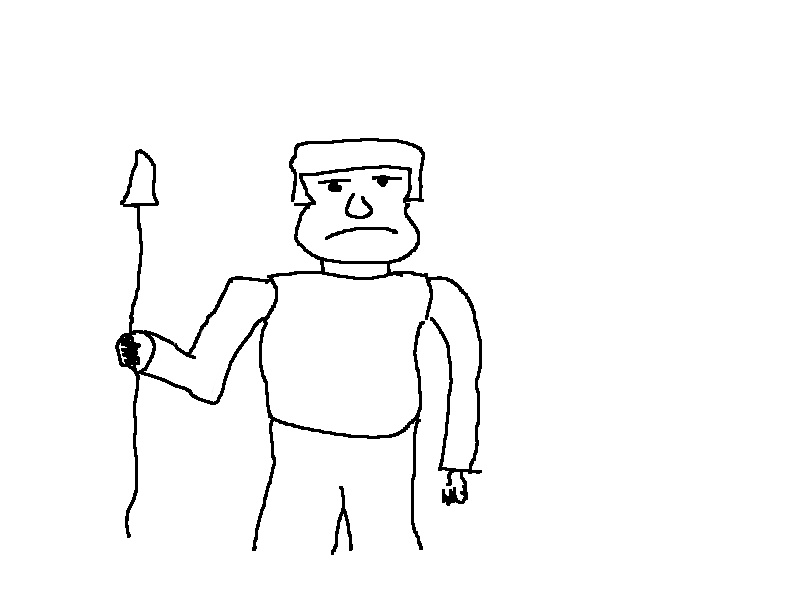
\includegraphics[width=5.0cm] {../img/card_img_H_Soldat.jpg}};}] (image) at (3.25,5.9375){};
\node (name) [text width=5.5cm, anchor=north west] at (0.5,8.5) {\titleofcard{Soldat}};
\node (level) at (3.25,0.5) {$\bigstar$};
\node (race) [draw, circle, fill=blue!40, minimum width=1cm, minimum height=1cm] at (5.8,8.3) {H$\mid$K};
\node (strength) [draw, circle, fill=white, anchor=east, minimum width=1cm, minimum height=1cm] at (6.3,7.0375) {\large2};
\node (actions) [draw, circle, fill=white, anchor=east, minimum width=1cm, minimum height=1cm] at (6.3,5.9375) {\large0};
\node (costs) [draw, circle, fill=white, anchor=east, minimum width=1cm, minimum height=1cm] at (6.3,4.8375) {\large7};
\node (rules) [text width=5.5cm, anchor=north west] at (0.4,2.775) {\begin{tabular}{l r}\textit{Schlachtformation}\end{tabular}};
\node (rows) [draw, circle, fill=white, minimum width=1cm, minimum height=1cm, path picture={\node [anchor=center]{
\includegraphics[width=1cm] {../img/symbol_sword.jpg}};}] at (1,3.375) {};

\node [draw, circle, fill=yellow!50, left=0.1cm of name] (desc_name) {A};
\node [draw, circle, fill=yellow!50, right=0.1cm of race] (desc_race) {B};
\node [draw, circle, fill=yellow!50, right=0.1cm of strength] (desc_str) {C};
\node [draw, circle, fill=yellow!50, right=0.1cm of actions] (desc_act) {D};
\node [draw, circle, fill=yellow!50, right=0.1cm of costs] (desc_cost) {E};
\node [draw, circle, fill=yellow!50, left=0.1cm of rows] (desc_rows) {F};
\node [draw, circle, fill=yellow!50, left=0.1cm of rules] (desc_rules) {G};
\node [draw, circle, fill=yellow!50, below=0.1cm of level] (desc_level) {H};

\end{tikzpicture}
\caption{Beispiel einer Spielkarte}\label{fig:karte}
\end{center}
\end{figure}

\subsubsection{Erläuterung der Karteneigenschaften}\label{sssec:Karteneigenschaften}
Eine Beispielkarte ist in \fref{fig:karte} gezeigt.
\paragraph{Kartenname}~\\
Der Kartenname dient dazu, die Karte zu identifizieren. Manche Sonderregeln gelten auch nur für Karten mit bestimmten Namen.
Der Kartenname ist ganz oben auf der Karte zu finden, siehe (A) in \fref{fig:karte}.

\paragraph{Volk und Fraktion}~\\
Das Volk und die Fraktion beschreiben das "Thema" des Decks. Volk und Fraktion sind im Kreis oben rechts auf der Karte durch ein eindeutiges Symbol bzw.\ durch eine Buchstabenkomination gekennzeichnet. Siehe (B) in \fref{fig:karte}.

Es gibt zur Zeit vier Völker (Menschen, Zwerge, Elfen und Monster), und je Volk zwei Fraktionen (z.\,B.\  Waldelfen und Hochelfen bei den Elfen). Alle Karten eines Decks müssen einer gemeinsamen Fraktion angehören (und damit natürlich auch zum selben Volk gehören).

Eine Ausnahme bilden die neutralen Karten, die jedoch auch nicht Teil des regulären Decks sind (dazu später mehr in \sref{ssec:Deck}).

\paragraph{Kartenlevel}~\\
Das Kartenlevel ist eine grobe Einteilung der Karten nach ihrer Stärke. Das Kartenlevel dient der Regulierung des Deckbaus, da die Anzahl hochleveliger Karten pro Deck beschränkt ist (dazu später mehr).
Das Level einer Karte wird auf zwei Arten gekennzeichnet. Es befinden sich am unteren Rand der Karte ein bis drei Sterne, deren Anzahl dem Kartenlevel entspricht (siehe (H) in \fref{fig:karte}). Außerdem zeigt die Anzahl der farbigen Rahmen um das Kartenbild sowie die Farbe der Rahmen das Kartenlevel (Level 1: Bronze, Level 2: Silber, Level 3: Gold).

Auch hier bilden die neutralen Karten eine Ausnahme: sie haben kein Kartenlevel.

\paragraph{Kartenstärke}~\\
Die Kartenstärke ist während des Spiels die wichtigste Eigenschaft der Karte, den sie bestimmt (abgesehen von Modifikationen durch Sonderregeln) den Punktwert der Karte am Rundenende. Die Kartenstärke ist im zweiten Kreis auf der rechten Seite notiert. Siehe (C) in \fref{fig:karte}.

\paragraph{Aktionspunkte}~\\
Die Aktionspunktzahl gibt an, wie viele Aktionspunkte die Karte beim Ausspielen erhält. Aktionspunkte sind wichtig für Karten, die wegen Sonderregeln \emph{Aktionen} ausführen können. Die Aktionspunktzahl ist im dritten Kreis auf der rechten Seite notiert, siehe (D) in \fref{fig:karte}.

\paragraph{Proviantkosten}~\\
Die Proviantkosten sind nur beim Zusammenstellen eines Decks wichtig und haben während des Spiels keine Bedeutung mehr. Diese Kosten beschreiben, wie "teuer" die Versorgung dieser Einheit für die Armee ist.
Das dient (ähnlich dem Kartenlevel) dem Balancing beim Deckbau, da die Summe der Proviantkosten aller Karten eines Kartendecks eine feste Grenze nicht überschreiten darf.
Die Aktionspunktzahl ist im vierten Kreis auf der rechten Seite notiert. Siehe (E) in \fref{fig:karte}.

Auch hier bilden die neutralen Karten eine Ausnahme: sie haben keine Proviantkosten.

\paragraph{Schlachtreihen}~\\
Die Schlachtreiehen unterteilen grob die verschiedenen Einheitentypen, und wie diese Truppen eingesetzt werden. Es gibt drei verschiedene Schlachtreiehen:

\begin{itemize}
	\item \textbf{Nahkampf}: wird gekennzeichnet durch zwei gekreuzte Schwerter: 
\includegraphics[height=0.6cm] {../img/symbol_sword.jpg}
	\item \textbf{Fernkampf}: wird gekennzeichnet durch Pfeil \& Bogen: 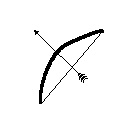
\includegraphics[height=0.6cm] {../img/symbol_bow.jpg}
	\item \textbf{Unterstützung}: wird gekennzeichnet durch eine Schriftrolle: 
\includegraphics[height=0.6cm] {../img/symbol_scroll.jpg}
\end{itemize}
Im Allgemeinen stehen Nahkämpfer in der vordersten Reihe, um in die feindliche Armee zu stürmen. In der zweiten Reihe stehen verschiedene Arten Fernkämpfer, die z.\,B.\ mit Pfeil und Bogen den Gegner aus der Distanz angreifen. Ganz hinten stehen schließlich die Generäle, die das Schlachtgeschehen überblicken und Befehle erteilen. Außerdem führen manche Armeen Belagerungswaffen mit großer Reichweite mit, die ebenfalls in der letzten Reihe aufgebaut werden.

Je nach Typ kann eine Einheit also nur in bestimmten Schlachtreihen eingesetzt werden. Welche Schlachtreihen das sind, ist durch Symbole unterhalb des Kartenbildes gekennzeichnet, siehe (F) in \fref{fig:karte}.

\paragraph{Sonderregeln}~\\
Schließlich haben die meisten Karten noch Sonderregeln, die das Spiel maßgeblich beeinflussen. Dazu mehr in \sref{ssec:Sonderregeln}. Die Namen der Sonderregeln einer Karte sind unterhalb ihrer Schlachreihen aufgelistet ((G) in \fref{fig:karte}); ihre Auswirkungen müssen auf einem seperaten Regelblatt nachgesehen werden.

\subsection{Sonderregeln}\label{ssec:Sonderregeln}
Es gibt \emph{passive} und \emph{aktive} Sonderregeln. Theoretisch kann eine Karte beliebig viele Sonderregeln haben, meistens liegt die Anzahl Sonderregeln einer Karte zwischen null und vier.
\begin{itemize}
	\item \emph{Passive Sonderregeln} (oder \emph{Eigenschaften}) sind gültig, solange sich die Einheit auf dem Spielfeld befindet und die Sonderregel nicht (in seltenen Fällen) von einer anderen Sonderregel explizit außer Kraft gesetzt wurde.\\
	Die passiven Sonderregeln einer Karte sind in \textit{kursiver Schrift} aufgelistet.
	\item \emph{Aktive Sonderregeln} (oder \emph{Aktionen}) unterscheiden sich in drei wesentlichen Punkten von den passiven Eigenschaften:
	\begin{itemize}
		\item Sie haben einmalige Effekte, die erst wirksam werden, wenn der kontrollierende Spieler sie während seines Zuges einsetzt.
		\item Das Einsetzen einer Aktion kostet Aktionspunkte (die \emph{Aktionskosten}), die aus dem Aktionspunktevorrat der ausführenden Karte bezahlt werden müssen.
		\item Die Aktion kann nur andere Karten beeinflussen, die ein gleichhohes oder niedrigeres Level als die ausführende Karte haben.
	\end{itemize}
	Ein Spieler kann eine Aktion von einer von ihm kontrollierten Karte jederzeit während seines eigenen Zuges auslösen (insbesondere müssen die Aktionen nicht beim Ausspielen der Karte ausgelöst werden!). Dafür entfernt er zuerst Aktionsmarker in Höhe der Aktionskosten von der ausführenden Karte, danach wird die beschriebene Aktion ausgeführt.\\
	Die aktiven Sonderregeln einer Karte sind in \textbf{fetter Schrift} aufgelistet.
	%Dafür müssen einige Bedingungen erfüllt sein. die Einheit noch über ausreichend Aktionspunkte (mindestens in Höhe der Aktionspunktkosten) verfügen. Vor dem Ausführen der Aktion muss die 
\end{itemize}

\subsubsection{Moralmodifikatoren}
Viele Sonderregeln bewirken \emph{Moralboni} oder \emph{Moralmali} für andere Karten.

\paragraph{Moralmarker}~\\
Diese Moralmodifikationen werden mit speziellen Markern individuell auf jeder Karte gekennzeichnet:
\begin{itemize}
	\item {\color{blue}\textbf{+}} für Moralboni
	\item {\color{red}\textbf{-}} für Moralmali.
\end{itemize}
Moralmarker sind immer an eine eindeutige Karte auf dem Spielfeld gebunden und dürfen nicht auf andere Einheiten verlegt werden.

Moralboni und -mali heben sich im Verhältnis 1:1 auf. Das bedeutet insbesondere, dass auf einer Karte nie gleichzeitig Moralmarker beider Arten liegen dürfen. 
Wir sagen, dass eine Karte mit mindestens einem Moralmalus \emph{negative Moral} hat; und analog hat eine Karte mit mindestens einem Moralbonus \emph{positive Moral}.

\paragraph{Effektive Kartenstärke}~\\
Die \emph{effektive Kartenstärke} ist die (aufgedruckte) Kartenstärke (siehe \sref{sssec:Karteneigenschaften}) plus die Summe ihrer Moralmodifikationsmarker.
%Am Ende einer Runde ist die \emph{effektive Kartenstärke} der Einheiten auf dem Spielfeld wichtig. Die effektive Kartenstärke ist die (aufgedruckte) Kartenstärke plus die Summe der Moralmodifikationsmarker der Karte.
Die effektive Kartenstärke kann nie kleiner sein als null. Das bedeutet, wenn die Anzahl der Moralmalus-Marker auf einer Karte ihrer Kartenstärke entspricht, kann sie keinen weiteren Moralmalus mehr erhalten. Jegliche Sonderregel, die dieser Karte einen weiteren Moralmalus hinzufügen würde, hat vorerst keine Wirkung. Natürlich kann die Karte immer noch Moralboni bekommen und dadurch wieder eine effektive Kartenstärke $> 0$ erhalten.

Solange eine Karte effektive Kartenstärke 0 hat, kann sie keine Aktionen einsetzen, und ihre passiven Eigenschaften haben vorerst keine Auswirkungen mehr.

\subsubsection{Sonstige Begriffe und Konventionen in den Definitionen der Sonderregeln}
\begin{itemize}
	\item Beim Ausführen einer Aktion und beim Umsetzen einer passiven Sonderregel wird diejenige Karte, welche die Regel ausgelöst hat, \emph{ausführende Karte} genannt. Alle Karten, die direkt von dieser Regel betroffen sind, werden \emph{betroffene Karten} genannt.
	\item Wann immer die \emph{Hälfte} von einem Wert genommen wird, ist der auf die nächste ganze Zahl \emph{abgerundete} Wert gemeint.
	\item \emph{Eigene} und \emph{verbündete} Einheiten bezeichnen Einheiten auf der eigenen Schlachtfeldseite. \emph{Gegnerische} Einheiten sind Einheiten auf der Schlachtfeldseite des Gegners.
	\item Einheiten sind \emph{adjazent} (oder \emph{benachbart}), wenn sie nebeneinander in der gleichen Schlachtreihe liegen.
	\item Die \emph{gegenüberliegende} Schlachtreihe einer Karte meint die Schlachtreihe, in der sich die Karte befindet, aber auf der Schlachtfeldseite des Gegners. D.\,h.\ es sind jeweils die beiden Nahkampf-Reihen, die beiden Fernkampf-Reihen sowie die beiden Unterstützer-Reihen \emph{gegenüberliegend}. 
	\item \emph{Token} sind Einheiten, die nicht Teil des Decks sind und nur durch Sonderregeln auf dem Schlachtfeld erscheinen können. Wenn sie das Schlachtfeld verlassen, werden sie nicht auf dem Ablagestapel abgelegt, sondern komplett aus dem Spiel entfernt. Tokens können auch nicht durch Sonderregeln auf die Hand genommen oder in den Nachziehstapel gemischt werden.
\end{itemize}

\subsection{Deck}\label{ssec:Deck}
\paragraph{Hauptdeck}~\\
Ein \emph{Deck} ist eine Menge von Karten mit folgenden Bedingungen:
\begin{itemize}
	\item Alle Karten gehören zu demselben Volk und zu derselben Fraktion.
	\item Das Deck besteht aus mindestens 25 Karten.
	\item Die Summe der Proviantkosten aller Karten im Deck übersteigt nicht 200.
	\item Das Deck enthält maximal 3 goldene Karten, und keine individuelle goldene Karte kommt doppelt vor.
    \item Das Deck enthält maximal 6 silberne Karten, und jede individuelle silberne Karte kommt höchstens zweimal vor.
    \item Jede individuelle bronzene Karte kommt höchstens viermal vor.
\end{itemize}
Hierbei sind \emph{individuelle} Karten solche mit identischem Kartennamen.

\paragraph{Sekundärdeck}~\\
Das \emph{Sekundärdeck} oder \emph{neutrale Deck} besteht aus exakt drei neutralen Karten oder Wetterkarten. Dies sind spezielle Karten, die keiner Fraktion angehören, kein Kartenlevel und keine Proviantkosten haben. %Das Sekundärdeck spielt eine besondere Rolle

\subsection{Spielbereiche}\label{ssec:Bereiche}
Während des Spiels sind die folgenden Spielbereiche und Kartenmengen relevant:
\begin{itemize}
	\item Nachziehstapel: verdeckt, und abgesehen von Sonderregeln nach Spielbeginn nicht mehr relevant. Der Nachziehstapel stellt quasi die Gesamtarmee der Fraktion des Spielers dar -- aber nicht alle Truppen sind in dieser Schlacht verfügbar.
	\item Hand: nur für den kontrollierenden Spieler jederzeit einsehbar (Nur durch Sonderregeln ggfs. auch für den Gegner). Die Hand eines Spielers ist die Armee, die er zur Verfügung hat.
	\item Ablagestapel: für beide Spieler jederzeit einsehbar. Dies sind die Truppen des Spielers, die in bereits vergangengen Runden eingesetzt wurden und nun erschöpft oder verwundet sind.
	\item Armeeaufstellungsbereich: bestehend aus drei \emph{Schlachtreihen}: \emph{Nahkampf}, \emph{Fernkampf} und \emph{Unterstützung}. Hier stellt der Spieler seine Truppe für das nächste Scharmüzel auf.
	\item gemeinsamer neutraler Nachziehstapel: verdeckt.
\end{itemize}
\fref{fig:Spiel} skizziert den Aufbau des Spielfeldes.

\begin{figure}
\begin{center}
\begin{center}
\begin{tikzpicture}
\draw [thick, dashed, fill=blue!10] (0,1.9) rectangle (12,7.95);
\draw [thick, dashed, fill=red!10] (0,8.05) rectangle (12,14.1);

% players side of board:
\draw [thick, dotted] (3, 6) rectangle (9, 7.8);
\draw [thick, dotted] (3, 4) rectangle (9, 5.8);
\draw [thick, dotted] (3, 2) rectangle (9, 3.8);

\draw [fill=blue!50] (5.1, 6.1) rectangle (5.9, 7.7) node[draw, circle, pos=.5, minimum width=0.7cm, minimum height=0.7cm, path picture={\node [anchor=center]{
\includegraphics[width=0.7cm] {../img/symbol_sword.jpg}};}] {}; 
\draw [fill=blue!50] (6.1, 6.1) rectangle (6.9, 7.7) node[draw, circle, pos=.5, minimum width=0.7cm, minimum height=0.7cm, path picture={\node [anchor=center]{
\includegraphics[width=0.7cm] {../img/symbol_sword.jpg}};}] {}; 

\draw [fill=blue!50] (4.6, 4.1) rectangle (5.4, 5.7) node[draw, circle, pos=.5, minimum width=0.7cm, minimum height=0.7cm, path picture={\node [anchor=center]{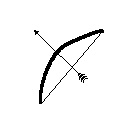
\includegraphics[width=0.7cm] {../img/symbol_bow.jpg}};}] {}; 
\draw [fill=blue!50] (5.6, 4.1) rectangle (6.4, 5.7) node[draw, circle, pos=.5, minimum width=0.7cm, minimum height=0.7cm, path picture={\node [anchor=center]{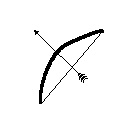
\includegraphics[width=0.7cm] {../img/symbol_bow.jpg}};}] {}; 
\draw [fill=blue!50] (6.6, 4.1) rectangle (7.4, 5.7) node[draw, circle, pos=.5, minimum width=0.7cm, minimum height=0.7cm, path picture={\node [anchor=center]{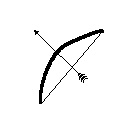
\includegraphics[width=0.7cm] {../img/symbol_bow.jpg}};}] {}; 

\draw [fill=blue!50] (5.6, 2.1) rectangle (6.4, 3.7) node[draw, circle, pos=.5, minimum width=0.7cm, minimum height=0.7cm, path picture={\node [anchor=center]{
\includegraphics[width=0.7cm] {../img/symbol_scroll.jpg}};}] {}; 

% players hand:
\draw [fill=blue!50, rotate around={-30:(6, 0.5)}] (5.6, 0.1) rectangle (6.4, 1.7) node[draw, circle, pos=.5, minimum width=0.7cm, minimum height=0.7cm, path picture={\node [anchor=center]{
\includegraphics[width=0.7cm] {../img/symbol_sword.jpg}};}] {}; 
\draw [fill=blue!50] (5.3, 0.1) rectangle (6.1, 1.7) node[draw, circle, pos=.5, minimum width=0.7cm, minimum height=0.7cm, path picture={\node [anchor=center]{
\includegraphics[width=0.7cm] {../img/symbol_sword.jpg}};}] {}; 
\draw [fill=blue!50,  rotate around={30:(5.4,0.5)}] (5, 0.1) rectangle (5.8, 1.7) node[draw, circle, pos=.5, minimum width=0.7cm, minimum height=0.7cm, path picture={\node [anchor=center]{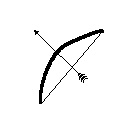
\includegraphics[width=0.7cm] {../img/symbol_bow.jpg}};}] {};

% players deck:
\draw [fill=blue!50] (10.1, 5.6) rectangle (10.9, 7.2) {};
\draw [fill=blue!50] (10.2, 5.7) rectangle (11, 7.3) {};
\draw [fill=blue!50] (10.3, 5.8) rectangle (11.1, 7.4) {};
\draw [fill=blue!50] (10.4, 5.9) rectangle (11.2, 7.5) {};
\draw [pattern=north west lines, pattern color=black!80] (10.4, 5.9) rectangle (11.2, 7.5) {};

% players discard pile:
\draw [fill=blue!50, rotate around={-10:(10.5,3.5)}] (10.1, 3.1) rectangle (10.9, 4.9) node[draw, circle, pos=.5, minimum width=0.7cm, minimum height=0.7cm, path picture={\node [anchor=center]{
\includegraphics[width=0.7cm] {../img/symbol_sword.jpg}};}] {}; 
\draw [fill=blue!50, rotate around={30:(10.5,3.5)}] (10.1, 3.1) rectangle (10.9, 4.9) node[draw, circle, pos=.5, minimum width=0.7cm, minimum height=0.7cm, path picture={\node [anchor=center]{
\includegraphics[width=0.7cm] {../img/symbol_sword.jpg}};}] {}; 
\draw [fill=blue!50, rotate around={-40:(10.5,3.5)}] (10.1, 3.1) rectangle (10.9, 4.9) node[draw, circle, pos=.5, minimum width=0.7cm, minimum height=0.7cm, path picture={\node [anchor=center]{
\includegraphics[width=0.7cm] {../img/symbol_sword.jpg}};}] {};

% opponents side of board:
\draw [thick, dotted] (3, 8.2) rectangle (9, 10);
\draw [thick, dotted] (3, 10.2) rectangle (9, 12);
\draw [thick, dotted] (3, 12.2) rectangle (9, 14);

\draw [fill=red!50] (4.1, 8.3) rectangle (4.9, 9.9) node[draw, circle, pos=.5, minimum width=0.7cm, minimum height=0.7cm, path picture={\node [anchor=center]{
\includegraphics[width=0.7cm] {../img/symbol_sword.jpg}};}] {}; 
\draw [fill=red!50] (5.1, 8.3) rectangle (5.9, 9.9) node[draw, circle, pos=.5, minimum width=0.7cm, minimum height=0.7cm, path picture={\node [anchor=center]{
\includegraphics[width=0.7cm] {../img/symbol_sword.jpg}};}] {}; 
\draw [fill=red!50] (6.1, 8.3) rectangle (6.9, 9.9) node[draw, circle, pos=.5, minimum width=0.7cm, minimum height=0.7cm, path picture={\node [anchor=center]{
\includegraphics[width=0.7cm] {../img/symbol_sword.jpg}};}] {}; 
\draw [fill=red!50] (7.1, 8.3) rectangle (7.9, 9.9) node[draw, circle, pos=.5, minimum width=0.7cm, minimum height=0.7cm, path picture={\node [anchor=center]{
\includegraphics[width=0.7cm] {../img/symbol_sword.jpg}};}] {}; 

\draw [fill=red!50] (5.6, 10.3) rectangle (6.4, 11.9) node[draw, circle, pos=.5, minimum width=0.7cm, minimum height=0.7cm, path picture={\node [anchor=center]{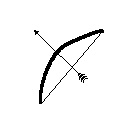
\includegraphics[width=0.7cm] {../img/symbol_bow.jpg}};}] {};

\draw [fill=red!50] (5.6, 12.3) rectangle (6.4, 13.9) node[draw, circle, pos=.5, minimum width=0.7cm, minimum height=0.7cm, path picture={\node [anchor=center]{
\includegraphics[width=0.7cm] {../img/symbol_scroll.jpg}};}] {}; 

% opponents hand:
\draw [fill=red!50, rotate around={30:(6,15.5)}] (5.6, 14.3) rectangle (6.4, 15.9){};
\draw [pattern=north west lines, pattern color=black!80, rotate around={30:(6,15.5)}] (5.6, 14.3) rectangle (6.4, 15.9){};
\draw [fill=red!50] (5.3, 14.3) rectangle (6.1, 15.9) {}; 
\draw [pattern=north west lines, pattern color=black!80] (5.3, 14.3) rectangle (6.1, 15.9) {}; 
\draw [fill=red!50, rotate around={-30:(5.4,15.5)}] (5, 14.3) rectangle (5.8, 15.9){};
\draw [pattern=north west lines, pattern color=black!80, rotate around={-30:(5.4,15.5)}] (5, 14.3) rectangle (5.8, 15.9){};

% opponents deck:
\draw [fill=red!50] (1.1, 9.1) rectangle (1.9, 10.7) {};
\draw [fill=red!50] (1.2, 9.2) rectangle (2, 10.8) {};
\draw [fill=red!50] (1.3, 9.3) rectangle (2.1, 10.9) {};
\draw [fill=red!50] (1.4, 9.4) rectangle (2.2, 11) {};
\draw [pattern=north west lines, pattern color=black!80] (1.4, 9.4) rectangle (2.2, 11) {}; 

% opponents discard pile:
\draw [fill=red!50, rotate around={10:(1.5, 12)}] (1.1, 11.5) rectangle (1.9, 13.3) node[draw, circle, pos=.5, minimum width=0.7cm, minimum height=0.7cm, path picture={\node [anchor=center]{
\includegraphics[width=0.7cm] {../img/symbol_scroll.jpg}};}] {}; 
\draw [fill=red!50, rotate around={-30:(1.5, 12)}] (1.1, 11.5) rectangle (1.9, 13.3) node[draw, circle, pos=.5, minimum width=0.7cm, minimum height=0.7cm, path picture={\node [anchor=center]{
\includegraphics[width=0.7cm] {../img/symbol_sword.jpg}};}] {}; 
\draw [fill=red!50, rotate around={50:(1.5, 12)}] (1.1, 11.5) rectangle (1.9, 13.3) node[draw, circle, pos=.5, minimum width=0.7cm, minimum height=0.7cm, path picture={\node [anchor=center]{
\includegraphics[width=0.7cm] {../img/symbol_scroll.jpg}};}] {};

% neutral deck:
\draw [fill=black!20] (12.5, 7.1) rectangle (13.3, 8.9)  node[draw, circle, pos=.5, minimum width=0.7cm, minimum height=0.7cm, path picture={\node [anchor=center]{
\includegraphics[width=0.7cm] {../img/symbol_weather.jpg}};}] {};

\draw [fill=black!20] (13.5, 7.1) rectangle (14.3, 8.9) {};
\draw [fill=black!20] (13.6, 7.2) rectangle (14.4, 9) {};
\draw [fill=black!20] (13.7, 7.3) rectangle (14.5, 9.1) {};
\draw [fill=black!20] (13.8, 7.4) rectangle (14.6, 9.2) {};
\draw [pattern=north west lines, pattern color=black!80] (13.8, 7.4) rectangle (14.6, 9.2) {};

\node [draw, circle, fill=yellow!50] at (0,3) {A1};
\node [draw, circle, fill=yellow!50] at (3,7) {A2};
\node [draw, circle, fill=yellow!50] at (3,5) {A3};
\node [draw, circle, fill=yellow!50] at (3,3) {A4};
\node [draw, circle, fill=yellow!50] at (10.4, 6.7) {A5};
\node [draw, circle, fill=yellow!50] at (10.1, 4.7) {A6};
\node [draw, circle, fill=yellow!50] at (5.5, 0.1) {A7};

\node [draw, circle, fill=yellow!50] at (12,13) {B1};
\node [draw, circle, fill=yellow!50] at (9,9) {B2};
\node [draw, circle, fill=yellow!50] at (9,11) {B3};
\node [draw, circle, fill=yellow!50] at (9,13) {B4};
\node [draw, circle, fill=yellow!50] at (2.2, 10.3) {B5};
\node [draw, circle, fill=yellow!50] at (1.9, 12.3) {B6};
\node [draw, circle, fill=yellow!50] at (5.8, 15) {B7};

\node [draw, circle, fill=yellow!50] at (13, 7.1) {C1};
\node [draw, circle, fill=yellow!50] at (14.6, 8.2) {C2};

\end{tikzpicture}
\end{center}
\caption{Skizze der Spielbereiche}\label{fig:Spiel}
Karten mit einem sichtbaren Schlachtreihen-Symbol liegen offen bzw.\ können vom Spieler jederzeit einsehen kann. Alle anderen Karten sind nicht einsehbar.
\end{center}
\begin{tabular}{l|l||l|l}
Label & Beschreibung & Label & Beschreibung \\ \hline
A1 & Spielbereich des Spielers & B1 & Spielbereich des Gegners\\
A2 & Nahkampf-Reihe des Spielers & B2 & Nahkampf-Reihe des Gegners \\
A3 & Fernkampf-Reihe des Spielers & B3 & Fernkampf-Reihe des Gegners \\
A4 & Support-Reihe des Spielers & B4 & Support-Reihe des Gegners \\
A5 & Nachziehstapel des Spielers & B5 & Nachziehstapel des Gegners \\
A6 & Ablagestapel des Spielers & B6 & Ablagestapel des Gegners \\
A7 & Handkarten des Spielers & B7 & Handkarten des Gegners \\ 
C1 & aktive Wettereffektkarten & & \\
C2 & Nachziehstapel des neutrales Decks & &
\end{tabular}

\end{figure}

\section{Spielablauf}
In einem Spiel spielen zwei Spieler mit vorher zusammengestellten Decks gegeneinander.
Ein Spiel besteht aus maximal drei Runden. Der Spieler, der zwei Runden gewinnt, gewinnt das Spiel.

In diesem Abschnitt wird der Ablauf des Spiels beschrieben. 

\subsection{Spielbeginn}
Zu Beginn des Spiels mischt jeder Spieler sein Deck und bildet dann daraus den verdeckten Nachziehstapel. Außerdem werden die Sekundärdecks beider Spieler vermischt, und daraus wird ein seperater verdeckter \emph{neutraler Nachziehstapel} gebildet.

Danach zieht jeder Spieler 10 Karten auf seine Hand, von denen bis zu zwei Karten abgeworfen und nachgezogen werden können. Im Fall, dass ein Spieler mindestens eine Karte nachgezogen hat, wird die abgeworfene Karte wieder in den Nachziehstapel gemischt. Schließlich einigen sich beide Spieler darauf, wer in der ersten Runde Startspieler ist (z.\,B.\ durch einen Münzwurf). Für alle weiteren Runden wechselt die Rolle des Startspielers mit jeder Runde.

\subsection{Spielrunden}
Eine Runde besteht daraus, dass beide Spieler abwechselnd (beginnend mit dem Startspieler) \emph{Spielzüge} ausführen, bis beide Spieler gepasst haben. Dann wird bestimmt, welcher Spieler die stärkere Armee aufgestellt hat und damit die Runde gewinnt.

Bevor der Startspieler seinen ersten Zug beginnt, zieht der \emph{Nicht-Startspieler} eine Karte vom neutralen Nachziehstapel.

\subsubsection{Spielzug}
Der Spieler, der an der Reihe ist, kann
\begin{itemize}
	\item \emph{entweder} einen Spielzug ausführen
	\item \emph{oder} passen.
\end{itemize}
Hat ein Spieler einmal gepasst, so passt er automatisch in allen weiteren Zügen in dieser Runde. Außerdem passt ein Spieler automatisch, sobald er keine Karten mehr auf der Hand hat.

Ein \emph{Spielzug} besteht \emph{immer} aus den folgenden Aktionen:
\begin{enumerate}
	\item \emph{Eine} Einheit von der Hand spielen. Dafür muss die Einheit in einer der Schlachreihen auf dem Spielfeld gelegt werden, die auch auf der Karte als mögliche Option angegeben sind. Beim Ausspielen einer Karte (und nur dann!) dürfen alle bereits ausliegenden Einheiten in der gespielten Schlachtreihe beliebig rearrangiert werden.
	\item Gegebenenfalls die Auswirkungen von passiven Eigenschaften von Karten auf dem Spielfeld beachten und befolgen. 
\end{enumerate}
Optional kann ein Spieler in seinem Zug:
\begin{itemize}
	\item beliebig viele Aktionen seiner Einheiten auslösen, solange die ausführenden Einheiten genügend Aktionspunkte zur Verfügung haben.
\end{itemize}

Zu Beachten: 
\begin{itemize}
	\item Während einer Runde werden keine Karten nachgezogen. Die Spieler müssen mit dem auskommen, was sie auf der Hand haben.
	\item Zwar kann ein Spieler auch eine Aktion auslösen, \emph{bevor} er eine Karte von seiner Hand spielt; allerdings kann er danach nicht mehr passen und \emph{muss} dann noch zwingend eine Karte ausspielen. 
	\item Ein Spieler, der keine Handkarten mehr besitzt, passt automatisch. Das bedeutet insbesondere, dass er dann auch keine Aktionen mehr ausführen kann.
\end{itemize}

\subsubsection{Rundenende}
Sobald beide Spieler gepasst haben, ist die Runde vorbei. Es werden nun noch alle passiven Eigenschaften ausgelöst, deren Effekte zum Rundenende in Kraft treten. Gibt es mehrere solcher Effekte,  treten sie in derselben Reihenfolge in Kraft, in der die Karten ursprünglich gespielt worden sind.
Anschließend wird für jeden Spieler die Summer der effektiven Kartenstärken aller Karten auf seiner Hälfte des Spielfeldes bestimmt. Der Spieler mit der höheren Gesamtstärke gewinnt die Runde.

\subsection{Spielende}
Sobald ein Spieler zwei Spielrunden gewonnen hat, ist das Spiel vorbei und dieser Spieler hat gewonnen.

\section{Alternative Regeln}
\begin{itemize}
	\item Nachschubregel: Zwischen den Runden werden die Armeen durch Nachschub verstärkt. Beide Spieler dürfen vor Beginn der zweiten und dritten Runde jeweils eine gewisse Anzahl an Karten (z.\,B. zwei Karten) nachziehen.
	\item Optional kann ohne ein neutrales Deck gespielt werden. Achtung: manche Sonderregeln werden dadurch wirkungslos, und Decks mit solchen Sonderregeln sind dann gegebenenfalls im Nachteil.
	\item Es ist auch denkbar, die Beschränkungen beim Deckbau anzupassen. Insbesondere die Gesamtproviantkosten und die Mindestkartenanzahl können an die eigenen Präferenzen angepasst werden. Wenn jedoch die Einschränkungen zur Kartenanzahl zu stark verändert werden, kann das weitreichende Auswirkungen auf das Spielbalancing haben.
\end{itemize}


\chapter{Erläuterungen zum Code}\label{ch:code}
Dieses Kapitel erklärt, wie eigene Fraktionen, Karten, Sonderregeln und Decks erstellt und dem Spiel hinzugefügt werden können. Außerdem wird der Python-Code dieses Projekts grob dokumentiert.

\section{Die Datenstruktur}
Sämtliche Karten, Sonderregeln sowie alle Völker und Fraktionen sind in xml-Dateien definiert. Dieses Projekt enthält einige Python-Skripte, die diese xml-Dateien parsen und daraus ausdruckbare Kartensets generieren können. Dadurch können Decks, Karten und sogar Sonderregeln oder Fraktionen sehr einfach variiert werden. Genauso einfach können auch komplett neue Decks, Karten, Sonderregeln und Fraktionen definiert werden.

\subsection{Definition der Fraktionen}
Die verschiedenen Fraktionen sind in der Datei \verb+xml/factions_definition.xml+ spezifiziert.

\subsection{Definition der Sonderregeln}
Sämtliche Sonderregeln sind in der Datei \verb+xml/rules.xml+ definiert.

\subsection{Definition der Karten}
Für jede Fraktion gibt es eine eigene Datei im Ordner \verb+xml/Factions/+, die die Definitionen für sämtliche Karten dieser Fraktion enthält. Der Dateiname ist dabei immer \verb+**_cards.xml+, wobei \verb+**+ für die jeweilige Fraktions-ID steht.

\subsection{Definition der Decks}
Die Decks sind jeweils durch eine eigene Datei im Ordner \verb+xml/Decks+ definiert.

\section{Ein Deck zusammenstellen}
Um ein eigenes Deck zusammenzustellen, muss eine xml-Datei im Ordner \verb+xml/Decks+ erstellt werden. Im Folgenden wird erläutert, wie diese Datei strukturiert sein muss und welche Daten sie enthalten muss. Im Allgemeinen sollten die in \sref{ssec:Deck} angegebenen Regeln eingehalten werden.

\subsection{Deckbeschreibung zusammenstellen}
Die xml-Datei des Decks muss die folgenden Komponenten enthalten:
\begin{itemize}
	\item \emph{Eine} Komponente mit dem Tag \verb+meta+. Diese Komponente muss die folgenden zwei Attribute beinhalten:
	\begin{itemize}
		\item \verb+main_faction_id+ : enthält die Fraktions-ID (siehe \verb+xml/factions_definitions.xml+) der Fraktion dieses Decks,
		\item \verb+name+ : beschreibt den Namen des Decks.
	\end{itemize}
	\item \emph{Beliebig viele} Komponenten mit dem Tag \verb+card+. Diese beschreiben alle Karten des Decks und enthalten jeweils die folgenden Attribute:
	\begin{itemize}
		\item \verb+faction_id+ : die ID der Fraktion, für welche diese Karte definiert ist,
		\item \verb+id+ : die ID der Karte, die in das Deck aufgenommen werden soll,
		\item \verb+amount+ : die Anzahl der Karte im Deck.
	\end{itemize}
\end{itemize}
Für Beispiele siehe die vorgegebenen Decks im Ordner \verb+xml/Decks+.

\subsection{Ausdruckdatei erzeugen}
Das Python-Skript \verb+deck_constructor.py+ erzeugt aus einer xml-Beschreibung eines Kartendecks eine pdf-Datei, die alle angegebenen Karten in ihrer spezifizierten Anzahl enthält. Falls einige der Karten Sonderregeln haben, durch die Tokens generiert werden können, so sind auch die entsprechenden Tokens in ausreichender Anzahl vorhanden. Außerdem enthält die pdf-Datei ein Regelblatt, auf dem alle Sonderregeln die auf Karten des Decks vorkommen erläutert sind.

Um mit diesem Skript eine Deck-pdf zu erzeugen, muss in der Konsole der Befehl
\begin{lstlisting}
python deck_constructor.py deck.xml
\end{lstlisting}
eingegeben werden, wobei \verb+deck.xml+ der Name der xml-Datei ist, die die Deckbeschreibung enthält. Diese Datei muss im Ordner \verb+xml/Decks+ liegen.

\subsection{Marker erzeugen}
Das Python-Skript \verb+maker_constructor.py+ erzeugt eine pdf-Datei, die jeweils 100 Moral+, Moral- und Aktionspunktemarker enthält. Einfach ausdrucken und ausschneiden.

Um mit diese pdf-Datei zu erzeugen, muss in der Konsole der Befehl
\begin{lstlisting}
python maker_constructor.py
\end{lstlisting}
eingegeben werden.

\section{Eigene Karten erstellen}\label{C:newcard}
Um eine eigene Karte für eine existierende Fraktion zu definieren, muss in der \verb+**_cards.xml+ der Fraktion eine neue \verb+card+-Komponente hinzugefügt werden. Eine solche Komponente muss die folgenden Attribute enthalten:
\begin{itemize}
	\item \verb+id+ : Die eindeutige ID der Karte. Wird benötigt, um die Karte in ein Deck aufzunehmen.
	\item \verb+name+ : Der Kartenname, der oben auf der Karte stehen wird.
	\item \verb+faction_id+ : Die Fraktion, zu der diese Karte gehört.
	\item \verb+level+ : Das Einheitenlevel.
	\item \verb+strength+ : Die Kartenstärke.
	\item \verb+actions+ : Die Anzahl der initialen Aktionspunkte.
	\item \verb+costs+ : Die Proviantkosten dieser Karte.
	\item \verb+image+ (optional) : Ein Dateiname (inklusive Endung) einer Bilddatei, die sich im Ordner \verb+img+ befindet. Wenn dieses Attribut auf eine valide Datei verlinkt, wird das Bild als Kartenbild eingebunden. Ansonsten wird das Default-Bild eines Schwertes verwendet.
\end{itemize}

Ferner sind die folgenden Child-Komponenten notwendig:
\begin{itemize}
	\item \verb+row+ (\emph{mindestens einmal}) : Beschreibt die Schlachtreihen, in der diese Karte gespielt werden kann. Diese Komponente \emph{muss} das Attribut \verb+name+ enthalten. Mögliche Werte für das \verb+name+-Attribut sind:
	\begin{itemize}
		\item \verb+CLOSE+ : Für die Nahkampfreihe
		\item \verb+RANGED+ : Für die Fernkampfreihe
		\item \verb+SUPPORT+ : Für die Unterstützungs- und Belagerungsreihe
		\item \verb+WEATHER+ (nur neutrale Karten) : Für die neutrale Wettereffekt-Reihe
	\end{itemize}
	\item \verb+rule+ (\emph{Optional}, maximal $5\times$) : Enthält die ID einer Sonderregel, die diese Karte haben soll. Diese Komponente \emph{muss} das Attribut \verb+id+ enthalten. Dieses Attribut wiederum muss eine ID einer Sonderregel enthalten, die in der Datei \verb+xml/rules.xml+ definiert ist.
\end{itemize}

\section{Eigene Sonderregeln hinzufügen}
Um neue Sonderregelen hinzuzufügen, muss in der Datei \verb+xml/rules.xml+ eine neue \verb+rule+-Komponente hinzugefügt werden.

\subsection{Sonderregeln allgemein}
Eine solche Komponente muss die folgenden Attribute enthalten:
\begin{itemize}
	\item \verb+id+ : Die eindeutige ID der Sonderregel. Diese ID wird verwendet, um diese Regel zu einer Karte hinzuzufügen.
	\item \verb+type+ : Beschreibt den Typus der Sonderregel. Muss entweder \verb+passive+ oder \verb+active+ sein.
	\item \verb+cost+ (nur für aktive Sonderregeln) : eine natürliche Zahl. Beschreibt die Aktionspunktekosten für das Ausführen dieser Regel.
	\item \verb+effekt+ : Ein Regeltext, der die Auswirkung dieser Sonderregel beschreibt.
\end{itemize}
Außerdem ist eine Child-Komponente \verb+label+ notwendig. Diese Komponente muss ein Attribut mit dem Namen jedes Volkes haben, das diese Sonderregel verwenden darf; der Wert der Attribute muss die entsprechende Bezeichnung der Regel für das Volk sein. Ein Beispiel: Angenommen, wir haben uns eine neue Regel ausgedacht; und nur Menschen oder Zwerge sollen diese Regel verwenden dürfen. Bei den Zwergen soll die Regel mit \emph{Grauer Bart} bezeichnet werden, aber bei Menschen soll die neue Regel \emph{Geschichtenerzähler} heissen. Dann muss die \verb+label+-Komponente die folgenden zwei Attribute erhalten:
\begin{itemize}
	\item \verb+Zwerge="Grauer Bart"+
	\item \verb+Menschen="Geschichtenerzähler"+
\end{itemize}
So ist es möglich, die Sonderregeln thematisch anzupassen. Außerdem kann eine Regel nicht einer Karte zugewiesen werden, wenn die Regel keine Bezeichnung für das Volk der Karte vorsieht. Damit wird sichergestellt, dass die Völker verschiedene Sets an Sonderregeln haben und so unterschiedliche Spieltaktiken ermöglichen.

\subsection{Token}
Bei Sonderregeln, die Token generieren können, müssen diese Token mittels einer Child-Komponente definiert werden.

TODO

\section{Eigene Völker und Fraktionen definieren}
Um ein eigenes Volk oder eine eigene Fraktion zu definieren, sind zwei Schritte notwendig.

\subsection{Einen Eintrag in der Fraktions-Definitionsdatei erstellen}
In der Datei \verb+xml/factions_definitions.xml+ muss für die neue Fraktion eine neue \verb+faction+ -Komponente erstellt werden. Diese Komponente muss die folgenden Attribute enthalten:
\begin{itemize}
	\item \verb+race_name+ : der Name des Volkes, zu dem die Fraktion gehört,
	\item \verb+faction_name+ : der Name der Fraktion,
	\item \verb+id+ : die ID dieser Fraktion, durch die sie überall sonst referenziert wird,
	\item \verb+color+ : die Farbe, die als Hintergrundfarbe für Karten dieser Fraktion verwendet wird. Diese Farbe muss entweder im \LaTeX -Paket \verb+graphicx+ enthalten sein, oder aber manuell in der template-Datei \verb+template.tex+ definiert werden.
\end{itemize}

\subsection{Eine neue Karten-Definitionsdatei erstellen und mit Karten füllen}
Im Ordner \verb+xml/Factions+ muss eine neue Datei mit dem Namen \verb+**_cards.xml+ erstellt werden (dabei ist \verb+**+ die Fraktions-ID der neuen Fraktion). In dieser Datei müssen Kartendefinitionen für alle Karten der neuen Fraktion hinzugefügt werden (siehe \sref{C:newcard}).

\section{Kartenübersicht in diesem Dokument aktualisieren}
Das Skript \verb+overview_constructor.py+ erzeugt für jede Fraktion einen \LaTeX -Code-Schnipsel, der jede Karte der Fraktion genau einmal darstellt. Dieser \LaTeX -Code wird automatisch beim Rekompilieren in dieses Dokument eingebunden (jedoch nur für die hier bereits enthaltenenen Völker und Fraktionen). 

Um mit die Fraktionsübersichten zu erzeugen, muss in der Konsole der Befehl
\begin{lstlisting}
python overview_constructor.py
\end{lstlisting}
eingegeben werden.

\section{Benötigte Software und Zusatzpackete}
\subsection{Python}
Der Python-Code ist für \verb+Python 3.7+ geschrieben und benötigt die folgenden Packages:
\begin{itemize}
	\item \verb+re+
	\item \verb+xml+
	\item \verb+os+
	\item \verb+sys+
	\item \verb+subprocess+
\end{itemize}

\subsection{\LaTeX}
Um ein eigenes Deck zu einer PDF-Datei zu kompilieren, wird \verb+pdflatex+ mit den folgenden Packages benötigt:
\begin{itemize}
	\item \verb+inputenc+
	\item \verb+geometry+
	\item \verb+pdflscape+
	\item \verb+tikz+
	\item \verb+graphicx+
	\item \verb+amsmath+
	\item \verb+amssymb+
	\item \verb+shellesc+
\end{itemize}

\chapter{Übersicht über Völker, Fraktionen und Karten}\label{ch:uebersicht}
in diesem Kapitel werden alle vorgegebenen Fraktionen vorgestellt. Für jede Fraktion werden alle existierenden Karten gezeigt und alle relevanten Sonderregeln angegeben.

Es ist zu beachten, dass die hier vorgestellten Karten im Allgemeinen nur als \emph{Vorschlag} oder \emph{Inspiration} gedacht sind. Die Fraktionen wurden noch nicht ausführlich getestet und es wird keine Garantie gegeben, dass die hier angegebenen Karten und Fraktionen ausgeglichene Spielstärke haben und zu spannenden Partien führen.

\section{Menschen}
\subsection{Kaiserreich}
\paragraph{Beschreibung}~\\
Der Kaiser der Menschen herrscht über ein großes Reich und verfügt über eine gutausgerüstete Armee. Ihre Kampfstrategie basiert auf starken Belagerungswaffen und zahlenmässige Überlegenheit. Außerdem verfügen sie über Spione, die hinter den feindlichen Linien wertvolle Informationen sammeln und die gegnerischen Anstrengungen sabotieren.

\paragraph{Übersicht aller Einheiten und Sonderregeln}~\\
\input{../tex/HK_puretikz_cards.tex}\\
\input{../tex/HK_puretikz_rules.tex}

\subsection{Heilige Armee}
\paragraph{Beschreibung}~\\
Die heilige Armee ist ein Zusammenschluss von gläubigen (oder beutegierigen) Rittern, die unter der Führung von Magiern und Geistlichen gegen alles Böse und Unheilige in den Kampf ziehen. Sie hoffen, durch ihren Kampf von den Göttern Vergebung für ihre Sünden zu erhalten.
Ihr starker Glaube gibt ihnen große Moralboni in der Schlacht.

\paragraph{Übersicht aller Einheiten und Sonderregeln}~\\
\input{../tex/HH_puretikz_cards.tex}\\
\input{../tex/HH_puretikz_rules.tex}


\section{Zwerge}
\subsection{Armee des Zwergenkönigs}
\paragraph{Beschreibung}~\\
Zwerge sind exzellente Nahkämpfer, die sich nicht so schnell einschüchtern lassen. Die Armee des Zwergenkönigs verfügt darüber hinaus über Ausrüstung und Belagerungswaffen allerhöchster Qualität.

\paragraph{Übersicht aller Einheiten und Sonderregeln}~\\
%(Nächste Seite)
%\includepdf[pages=-,pagecommand={}]{../pdf/DR.pdf}
\input{../tex/ZK_puretikz_cards.tex}\\
\input{../tex/ZK_puretikz_rules.tex}


\subsection{Wilde Zwerge}
\paragraph{Beschreibung}~\\
Die Wilden Zwerge sind ein verstreut lebendes Volk, das dem rauen Klima im hohen Norden trotzt. Zwar sind sie weniger gut ausgerüstet als die Armee des Zwergenkönigs, aber das gleichen sie durch ihre Wildheit und Zähigkeit wieder aus.

\paragraph{Übersicht aller Einheiten und Sonderregeln}~\\
\input{../tex/ZW_puretikz_cards.tex}\\
\input{../tex/ZW_puretikz_rules.tex}


\section{Elfen}
\subsection{Hochelfen}
\paragraph{Beschreibung}~\\
Die Hochelfen sind ein altes und magisches Volk, die ihre Gegner allein durch ihre Anwesenheit einschüchtern. Wenn es zum Kampf kommt, sind diese Elfen beinahe unaufhaltsame Kampfmaschinen, und ihr unvergleichliches Wissen über alle Dinge verleiht ihnen noch manch zusätzlichen Vorteil.

\paragraph{Übersicht aller Einheiten und Sonderregeln}~\\
\input{../tex/EH_puretikz_cards.tex}\\
\input{../tex/EH_puretikz_rules.tex}


\subsection{Waldelfen}
\paragraph{Beschreibung}~\\
Waldelfen sind nicht weniger mächtig als ihre Verwandten; aber sie bevorzugen Kampftaktiken, die auf Heimlichkeit beruhen. Sie überziehen ihre Gegner mit Sabotageaktioen und Überfällen. Außerdem sind sie eins mit der Natur und können sich auf die Hilfe von guten Geistern und manchen wilden Tieren verlassen.

\paragraph{Übersicht aller Einheiten und Sonderregeln}~\\
%(Nächste Seite)
%\includepdf[pages=-,pagecommand={}]{../pdf/EW.pdf}
\input{../tex/EW_puretikz_cards.tex}\\
\input{../tex/EW_puretikz_rules.tex}

\section{Monster}
\subsection{Wilde Bestien}
\paragraph{Beschreibung}~\\
Manchmal versammeln sich die Monster und Tiere der Wildnis um ein besonders mächtiges Biest und greifen gemeinsam die anderen Völker an. Solch eine Rotte stellt auch für eine gutausgerüstete Armee ein ernstes Problem dar. Nicht nur sind manche Bestien von furchterregender Größe und Macht unter Ihnen; wegen ihre Wildheit und Zähigkeit sind sie auch schwer mit herkömmlichen Armeetaktiken zu bezwingen. Außerdem werden durch die Schreie der wilden Tiere während des Kampfes häufig noch weitere Tiere angelockt.

\paragraph{Übersicht aller Einheiten und Sonderregeln}~\\
\input{../tex/MB_puretikz_cards.tex}\\
\input{../tex/MB_puretikz_rules.tex}

\subsection{Geister}
\paragraph{Beschreibung}~\\
Auf alten Friedhöfen, in verfallenen Burgruinen und an ehemaligen Schlachtfeldern existieren zahllose verfluchte Wesen wie Untote, Geister und Vampire. Mächtigen Schwarzmagiern oder Vampirfürsten gelingt es von Zeit zu Zeit, eine größere Menge dieser Wesen unter ihre Kontrolle zu zwingen. Diese Truppen verbreiten dann Terror und Horror wo immer sie auftauchen; und ihre Gegner sind meist schon vor dem Kampf vor Angst erschöpft.

\paragraph{Übersicht aller Einheiten und Sonderregeln}~\\
\input{../tex/MG_puretikz_cards.tex}\\
\input{../tex/MG_puretikz_rules.tex}

\section{Neutrale Karten}
\subsection{Wetterkarten}
\paragraph{Beschreibung}~\\
(TO DO)

\paragraph{Übersicht aller Einheiten und Sonderregeln}~\\
\input{../tex/NW_puretikz_cards.tex}\\
\input{../tex/NW_puretikz_rules.tex}

\subsection{Fahrende Ritter}
\paragraph{Beschreibung}~\\
(TO DO)

\paragraph{Übersicht aller Einheiten und Sonderregeln}~\\
\input{../tex/NR_puretikz_cards.tex}\\
\input{../tex/NR_puretikz_rules.tex}

\chapter{Mögliche Erweiterungen und Alternativen}
Beim Ausdenken neuer Völker, Decks und Karten sind der Fantasie prinzipiell keine Grenzen gesetzt. Die klassischen Fantasy-Universen lassen sich gut zur Inspiration heranziehen.

An dieser Stelle muss der kreative Prozess aber noch nicht enden. Es ist auch denkbar, ein komplett neues Setting einzuführen. Keine Lust auf Fantasy? Das Spielprinzip funktioniert grundsätzlich auch im Weltkriegsszenario. Hier müssten natürlich fast alle Regeln und Begriffe umbenannt werden; z.\,B.\ \emph{Nahkampf} zu \emph{Infanterie}, \emph{Fernkampf} zu \emph{Artillerie} und \emph{Support} zu \emph{Spionage} oder \emph{Luftwaffe}. Genauso ist auch ein Science-Fiction-Setting mit Weltraumkämpfen denkbar.

Die Begrifflichkeiten können auch soweit abgewandelt werden, dass es im Spiel gar nicht mehr um einen direkten \emph{Kampf} geht, sondern ganz allgemeinen um einen \emph{Wettstreit}, bei dem es in drei Runden jeweils in drei Kategorien Punkte zu holen gibt. Ein solches Setting soll ihr zur Inspiration kurz umrissen werden.

\paragraph{Beispiel eines alternativen Settings: Wettstreit zweier Festivalveranstalter}~\\
Die Spieler sind jeweils Veranstalter eines mehrtägigen (Musik-)Festivals. Das Spiel geht über drei Runden, wobei jede Runde einem Festivaltag entspricht. In jeder Runde versuchen die Spieler ihren Festivaltag möglichst stimmungsvoll zu gestalten, in dem sie Karten in den Kategorien \emph{Bühne} (entspricht der Nahkampf-Reihe), \emph{Merchandise} (entspricht der Fernkampf-Reihe) und \emph{Zeltplatz} (entspricht der Support-Reihe) ausspielen. Anstatt verschiedener Völker gibt es verschiedene Festival-Typen, die unterschiedliche Spielmechaniken ermöglichen (z.\,B.\ ,,Metal-Festival'' oder ,,Alternatives Festival'').

\end{document}